% =============================================================================
% ISAIS 2026 Research-in-Progress Paper
% Graph-Based Earnings Manipulation Detection
% =============================================================================
\documentclass[12pt,a4paper]{article}

% --- Packages ----------------------------------------------------------------
\usepackage[utf8]{inputenc}
\usepackage[T1]{fontenc}
\usepackage{mathptmx}                    % Times New Roman
\usepackage[margin=1in]{geometry}
\usepackage{setspace}\doublespacing       % Double-spaced (standard AIS format)
\usepackage{amsmath,amssymb}
\usepackage{graphicx}
\usepackage{booktabs}
\usepackage{tabularx}
\usepackage{multirow}
\usepackage{caption}
\usepackage{subcaption}
\usepackage{float}
\usepackage{hyperref}
\hypersetup{colorlinks=true,linkcolor=blue,citecolor=blue,urlcolor=blue}
\usepackage[numbers]{natbib}              % Author-year citations
\usepackage{algorithm}
\usepackage{algpseudocode}
\usepackage{tikz}
\usetikzlibrary{shapes,arrows,positioning,fit,backgrounds}

% --- Custom commands ---------------------------------------------------------
\newcommand{\todo}[1]{\textcolor{red}{\textbf{[TODO: #1]}}}
\newcommand{\placeholder}[1]{\textcolor{blue}{\textbf{[#1]}}}

% =============================================================================
\begin{document}

% --- Title Block -------------------------------------------------------------
\begin{center}
{\LARGE\bfseries Graph-Based Financial Statement Analysis for Detecting\\[4pt]
Earnings Manipulation: An Explainable AI Approach}

\vspace{18pt}

{\large Research-in-Progress}

\vspace{18pt}

{\large
Apoorv Saxena\\[4pt]
College of Management, Yuan Ze University, Taoyuan, Taiwan\\[2pt]
s1129420@mail.yzu.edu.tw
}

\vspace{12pt}

{\large
Yan-Jie Yang\textsuperscript{*}\\[4pt]
College of Management, Yuan Ze University, Taoyuan, Taiwan\\[2pt]
yanjie@saturn.yzu.edu.tw
}

\vspace{6pt}
{\small \textsuperscript{*}Corresponding author.}

\vspace{18pt}

\textit{Submitted to the 14th International Symposium on\\
Accounting Information Systems (ISAIS 2026)}

\vspace{6pt}

March 2026

\end{center}

\newpage

% =============================================================================
\section*{Abstract}
% =============================================================================

Traditional earnings manipulation detection methods, such as the Beneish M-Score and Dechow F-Score, analyze financial ratios independently, treating each indicator as an isolated signal. However, earnings manipulation---whether through accrual-based earnings management (AEM) or real activities manipulation (REM)---is fundamentally a relational phenomenon: manipulation in one account propagates strain across interconnected financial statement relationships. We propose a \textit{graph-based} detection framework that models financial statements as a \textit{vulnerability graph}, a directed network in which nodes represent financial accounts and ratios, and edges encode the expected accounting relationships between them. Deviations from expected relationships are quantified as edge strain using industry-adjusted $z$-scores, and graph-theoretic metrics (PageRank, betweenness centrality) identify the accounts most central to manipulation patterns. We combine the graph-based risk score with traditional methods in a weighted ensemble and layer an explainable AI component---a local large language model (LLM) augmented with historical fraud case retrieval---to produce natural-language audit narratives. We validate our approach on the JarFraud dataset, which contains SEC Accounting and Auditing Enforcement Release (AAER) labels. Preliminary results from stratified cross-validation indicate that the graph-enhanced ensemble \placeholder{outperforms / matches} individual traditional methods in AUC-ROC, while providing auditors with interpretable, relationship-level explanations of flagged anomalies. This research-in-progress contributes to the accounting information systems literature by demonstrating how graph analytics can operationalize the theoretical insight that earnings manipulation distorts \textit{relationships} among accounts, not merely individual ratios.

\vspace{6pt}
\noindent\textbf{Keywords:} Earnings manipulation detection, vulnerability graph, accrual earnings management, real activities manipulation, explainable AI, graph analytics, forensic accounting, JarFraud

% =============================================================================
\section{Introduction}
\label{sec:intro}
% =============================================================================

Financial statement fraud remains one of the most costly and challenging problems in capital markets. The Association of Certified Fraud Examiners (ACFE) estimates that organizations lose approximately 5\% of annual revenue to fraud, with financial statement fraud producing the largest median losses per incident \cite{acfe2024}. Despite advances in auditing standards and regulatory oversight, high-profile scandals---from Enron and WorldCom to more recent cases such as Wirecard---underscore the persistent difficulty of detecting earnings manipulation in a timely manner.

Academic research has responded with a rich portfolio of statistical models. The Beneish M-Score \cite{beneish1999} uses financial ratio analysis to flag firms likely to have manipulated earnings through accrual-based techniques. The Dechow F-Score \cite{dechow2011} extends this approach by incorporating accrual quality measures derived from the Richardson et al.\ \cite{richardson2005} RSST accrual decomposition, soft-asset ratios, and changes in receivables. More recently, machine learning methods---random forests, gradient boosting, neural networks---have been applied to fraud detection with promising results \cite{bao2020,cecchini2010}. However, these data-driven approaches often function as ``black boxes,'' producing predictions without the interpretable audit trail that practitioners require.

A critical gap in all these approaches is their treatment of financial accounts as \textit{independent} variables. In practice, financial statements are a system of interconnected accounts governed by double-entry bookkeeping, industry-specific operating cycles, and accrual accounting rules. When a firm manipulates earnings, the manipulation rarely distorts a single ratio in isolation; instead, it creates \textit{strain} that propagates across related accounts. For example, revenue inflation through premature recognition simultaneously distorts the revenue-to-receivables relationship (elevated days sales outstanding), the revenue-to-cash-flow relationship (diverging operating cash flows), and the accrual-to-income relationship (increasing discretionary accruals). Traditional methods may detect each symptom separately, but they do not model the \textit{relational structure} that connects them.

This relational perspective is especially important in light of the well-documented phenomenon of \textit{AEM--REM substitution}. Cohen et al.\ \cite{cohen2008} and Zang \cite{zang2012} demonstrate that firms strategically substitute between accrual-based earnings management and real activities manipulation in response to varying constraints---regulatory scrutiny, audit quality, litigation risk. When accrual manipulation becomes costly (e.g., after SOX), firms shift toward real activities such as overproduction, discretionary expense cuts, or channel stuffing. This substitution is inherently a \textit{relational} phenomenon: pressure that cannot flow through one manipulation channel is redirected to another. A detection system that analyzes each channel independently will miss the substitution pattern.

In this research-in-progress paper, we propose a \textit{graph-based earnings manipulation detection framework} that addresses these limitations. Our approach makes three contributions:

\begin{enumerate}
    \item \textbf{Vulnerability graph model.} We model financial statements as directed graphs in which nodes represent financial accounts and ratios, and weighted edges represent the expected relationships between them (e.g., the expected ratio of revenue to cost of goods sold, or of net income to operating cash flow). Edge weights encode industry-adjusted statistical expectations, and deviations from these expectations are quantified as \textit{edge strain} using $z$-scores. Graph-theoretic metrics---PageRank, betweenness centrality, and path-based strain propagation---identify accounts that are central to manipulation patterns. This operationalizes the theoretical insight that manipulation distorts \textit{relationships}, not merely individual ratios.

    \item \textbf{Ensemble integration with traditional methods.} We combine the graph-based risk score with Beneish M-Score and Dechow F-Score in a weighted ensemble, leveraging the complementary strengths of relational analysis (graph) and established ratio-based methods (Beneish, Dechow). We validate the ensemble on the JarFraud dataset \cite{bao2020} with stratified cross-validation, reporting AUC-ROC, precision, recall, and F1-score.

    \item \textbf{Explainable AI layer.} We integrate a local large language model (DeepSeek-R1) with retrieval-augmented generation (RAG) over a database of historical SEC enforcement cases, enabling the system to produce natural-language audit narratives that explain \textit{why} a firm was flagged, \textit{which} account relationships are strained, and \textit{how} the pattern compares to historical fraud cases. This addresses the ``black-box'' criticism of machine learning approaches in auditing.
\end{enumerate}

The remainder of this paper is organized as follows. Section~\ref{sec:lit} reviews the relevant literature on earnings manipulation detection, AEM--REM substitution, and graph analytics in accounting. Section~\ref{sec:method} describes our research design and the technical architecture of the framework. Section~\ref{sec:results} presents preliminary results. Section~\ref{sec:discuss} discusses implications and limitations, and Section~\ref{sec:conclude} outlines planned future work.

% =============================================================================
\section{Literature Review}
\label{sec:lit}
% =============================================================================

\subsection{Earnings Manipulation Detection}

The detection of earnings manipulation has evolved through three broad phases. The first phase, rooted in analytical procedures, produced ratio-based models such as Beneish's \cite{beneish1999} M-Score, which combines eight financial ratios---days' sales in receivables index (DSRI), gross margin index (GMI), asset quality index (AQI), sales growth index (SGI), depreciation index (DEPI), sales general and administrative expenses index (SGAI), leverage index (LVGI), and total accruals to total assets (TATA)---into a discriminant function calibrated on known fraud firms. Dechow et al.\ \cite{dechow2011} extended this approach with the F-Score, incorporating RSST accruals, changes in receivables, and soft-asset ratios, and demonstrated that the F-Score improved upon the M-Score in out-of-sample tests.

The second phase introduced machine learning methods. Cecchini et al.\ \cite{cecchini2010} applied support vector machines to SEC filings, while Bao et al.\ \cite{bao2020} demonstrated that ensemble methods (RUSBoost) trained on the JarFraud dataset---a comprehensive panel of SEC AAER-labeled observations---substantially outperformed logistic regression baselines. Subsequent work explored deep learning \cite{craja2020}, textual analysis of MD\&A disclosures, and anomaly detection algorithms. While these methods achieve strong predictive performance, they share two limitations: (i) they treat financial variables as independent features rather than elements of a relational system, and (ii) they lack interpretability, making it difficult for auditors to act on their predictions.

The third phase, still emerging, seeks to combine predictive accuracy with \textit{explainability}. Our work falls within this phase, proposing graph-based analysis as a mechanism that is both relationally aware and inherently interpretable.

\subsection{AEM--REM Substitution}

A foundational insight in the earnings management literature is that firms do not rely on a single manipulation technique. Accrual-based earnings management (AEM) involves discretionary adjustments to accruals---for example, delaying bad-debt write-offs or recognizing revenue prematurely---without changing underlying real transactions. Real activities manipulation (REM), by contrast, involves altering actual business decisions---overproduction to reduce per-unit cost of goods sold, cutting discretionary expenditures, or granting price discounts to accelerate revenue recognition \cite{roychowdhury2006}.

Cohen et al.\ \cite{cohen2008} provide evidence that AEM declined and REM increased after the passage of the Sarbanes-Oxley Act (SOX), suggesting that firms substituted away from accrual manipulation as regulatory scrutiny intensified. Zang \cite{zang2012} formalizes this substitution as a sequential decision: firms first choose a level of REM early in the fiscal year and then adjust AEM at year-end based on the realized cost of accrual manipulation. Subsequent research \cite{cohen2010,ho2015} has refined this model, identifying firm-specific moderators such as auditor quality, industry competition, and institutional ownership.

The substitution phenomenon has direct implications for fraud detection: a system that monitors only accrual-based indicators (e.g., Beneish M-Score) may fail to detect a firm that has shifted manipulation to real activities, and vice versa. Our graph-based approach addresses this by modeling \textit{both} AEM and REM indicators as nodes in a unified vulnerability graph, where the relationships between them capture the substitution dynamics.

\subsection{Graph Analytics in Accounting and Finance}

Graph-based methods have gained traction in financial applications, primarily in the domains of money laundering detection \cite{savage2016}, insider trading networks \cite{ahern2017}, and supply chain risk analysis. In accounting, Dechow et al.\ \cite{dechow2011} implicitly acknowledged the relational nature of financial statements by modeling accrual quality through the interaction between receivables, cash flows, and income, but did not formalize this structure as a graph.

More recently, graph neural networks (GNNs) have been applied to fraud detection in transaction networks \cite{liu2021,wang2019}, where nodes represent entities (e.g., bank accounts) and edges represent transactions. However, these approaches model \textit{inter-entity} networks (who transacts with whom), not \textit{intra-entity} financial statement relationships (how accounts within a single firm relate to each other). Our vulnerability graph model is, to our knowledge, among the first to apply graph analytics to the \textit{internal} structure of financial statements for manipulation detection.

% =============================================================================
\section{Research Design}
\label{sec:method}
% =============================================================================

\subsection{Overview}

Our framework consists of four components: (1) a vulnerability graph that models financial statement relationships, (2) graph-based anomaly detection using industry-adjusted $z$-scores and network metrics, (3) an ensemble that combines the graph-based risk score with traditional Beneish and Dechow scores, and (4) an explainable AI layer that generates natural-language audit narratives. Figure~\ref{fig:architecture} illustrates the pipeline.

\begin{figure}[H]
\centering
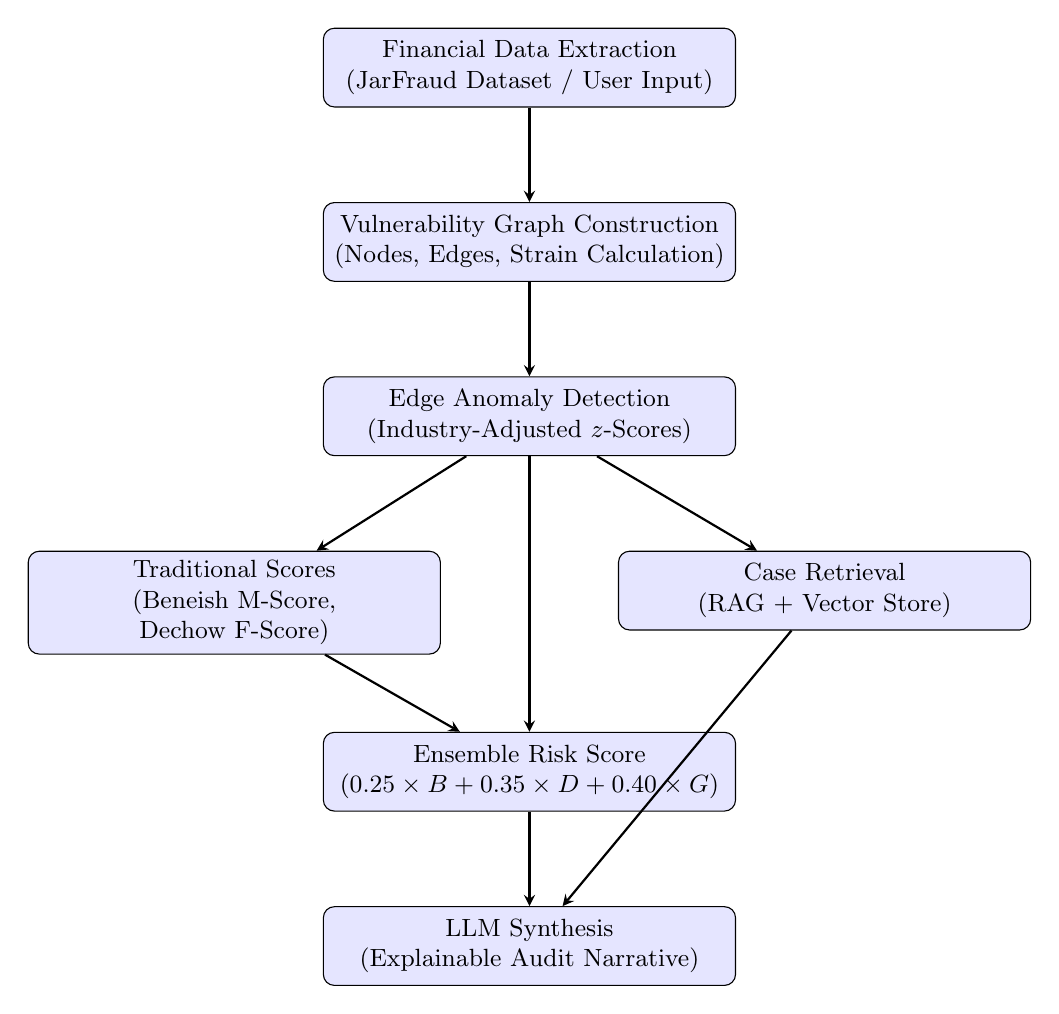
\begin{tikzpicture}[
    node distance=1.2cm and 2cm,
    block/.style={rectangle, draw, fill=blue!10, text width=5cm, text centered, rounded corners, minimum height=1cm, font=\small},
    arrow/.style={->, thick, >=stealth}
]
\node[block] (data) {Financial Data Extraction\\(JarFraud Dataset / User Input)};
\node[block, below=of data] (graph) {Vulnerability Graph Construction\\(Nodes, Edges, Strain Calculation)};
\node[block, below=of graph] (anomaly) {Edge Anomaly Detection\\(Industry-Adjusted $z$-Scores)};
\node[block, below left=1.2cm and -1.5cm of anomaly] (trad) {Traditional Scores\\(Beneish M-Score, Dechow F-Score)};
\node[block, below right=1.2cm and -1.5cm of anomaly] (rag) {Case Retrieval\\(RAG + Vector Store)};
\node[block, below=3.5cm of anomaly] (ensemble) {Ensemble Risk Score\\($0.25 \times B + 0.35 \times D + 0.40 \times G$)};
\node[block, below=of ensemble] (llm) {LLM Synthesis\\(Explainable Audit Narrative)};

\draw[arrow] (data) -- (graph);
\draw[arrow] (graph) -- (anomaly);
\draw[arrow] (anomaly) -- (trad);
\draw[arrow] (anomaly) -- (rag);
\draw[arrow] (trad) -- (ensemble);
\draw[arrow] (anomaly) -- (ensemble);
\draw[arrow] (rag) -- (llm);
\draw[arrow] (ensemble) -- (llm);
\end{tikzpicture}
\caption{System architecture: from financial data to explainable audit narrative.}
\label{fig:architecture}
\end{figure}

\subsection{Vulnerability Graph Construction}
\label{subsec:graph}

We model a firm's financial statements as a directed graph $G = (V, E)$, where:

\begin{itemize}
    \item \textbf{Nodes} $V = V_A \cup V_R \cup V_G$ comprise three types:
    \begin{itemize}
        \item \textit{Account nodes} ($V_A$): revenue, cost of goods sold (COGS), gross profit, operating income, net income, accounts receivable, inventory, accounts payable, property plant and equipment (PP\&E), and total assets.
        \item \textit{Ratio nodes} ($V_R$): days sales outstanding (DSO), days inventory outstanding (DIO), days payable outstanding (DPO), and cash conversion cycle.
        \item \textit{Governance nodes} ($V_G$): auditor type and auditor tenure (when available).
    \end{itemize}
    \item \textbf{Edges} $E$ connect nodes that have a known accounting relationship, with each edge $e_{ij} \in E$ carrying an expected ratio $\mu_{ij}$ and standard deviation $\sigma_{ij}$ based on industry benchmarks (Table~\ref{tab:edges}).
\end{itemize}

\begin{table}[H]
\centering
\caption{Core edges in the vulnerability graph with industry-default expectations.}
\label{tab:edges}
\small
\begin{tabular}{llccc}
\toprule
\textbf{Source} & \textbf{Target} & \textbf{Type} & $\boldsymbol{\mu}$ & $\boldsymbol{\sigma}$ \\
\midrule
Revenue      & COGS           & Identity    & 0.65 & 0.05 \\
Revenue      & Accts.\ Recv.\ & Identity    & 0.08 & 0.02 \\
COGS         & Inventory      & Identity    & 0.25 & 0.05 \\
COGS         & Accts.\ Pay.\  & Identity    & 0.10 & 0.03 \\
Revenue      & Gross Profit   & Identity    & 0.35 & 0.05 \\
Gross Profit & Operating Inc. & Correlation & 0.60 & 0.10 \\
Operating Inc.& Net Income    & Correlation & 0.75 & 0.15 \\
\bottomrule
\end{tabular}
\end{table}

For each edge, \textit{edge strain} is computed as:
\begin{equation}
\text{Strain}(e_{ij}) = \frac{|r_{ij} - \mu_{ij}|}{\sigma_{ij}},
\label{eq:strain}
\end{equation}
where $r_{ij}$ is the observed ratio between the source and target node values. Edge strain exceeding 2.0 standard deviations is classified as \textsc{broken}; between 1.0 and 2.0 as \textsc{stressed}; and below 1.0 as \textsc{intact}.

\subsection{Edge Anomaly Detection with Industry-Adjusted \texorpdfstring{$z$}{z}-Scores}
\label{subsec:anomaly}

Beyond generic strain, we apply industry-adjusted $z$-scores to four diagnostically critical edges that capture both AEM and REM pathways:

\begin{enumerate}
    \item \textbf{Revenue $\to$ Operating Cash Flow} (Cash Quality):
    \begin{equation}
        z_{\text{CFO}} = \frac{(\text{CFO}/\text{Revenue}) - \mu_{\text{CFO}}^{(k)}}{\sigma_{\text{CFO}}^{(k)}},
    \end{equation}
    where $\mu_{\text{CFO}}^{(k)}$ and $\sigma_{\text{CFO}}^{(k)}$ are industry-group benchmarks indexed by SIC code group $k$. A strongly negative $z_{\text{CFO}}$ signals revenue that does not convert to cash---a hallmark of premature revenue recognition (AEM).

    \item \textbf{Revenue $\to$ Accounts Receivable} (Collection Quality):
    \begin{equation}
        z_{\text{DSO}} = \frac{\text{DSO} - \mu_{\text{DSO}}^{(k)}}{\sigma_{\text{DSO}}^{(k)}},
    \end{equation}
    where $\text{DSO} = (\text{AR}/\text{Revenue}) \times 365$. Elevated DSO (positive $z$) suggests receivables growing faster than revenue---a channel-stuffing or fictitious-revenue signal.

    \item \textbf{COGS $\to$ Inventory} (Production Efficiency):
    \begin{equation}
        z_{\text{DIO}} = \frac{\text{DIO} - \mu_{\text{DIO}}^{(k)}}{\sigma_{\text{DIO}}^{(k)}},
    \end{equation}
    where $\text{DIO} = (\text{Inventory}/\text{COGS}) \times 365$. Elevated DIO signals overproduction to spread fixed costs---a classic REM technique identified by Roychowdhury \cite{roychowdhury2006}.

    \item \textbf{Net Income $\to$ Operating Cash Flow} (Accrual Quality):
    \begin{equation}
        z_{\text{Accrual}} = \frac{(\text{NI} - \text{CFO})/\text{TA} - \mu_{\text{Acc}}^{(k)}}{\sigma_{\text{Acc}}^{(k)}},
    \end{equation}
    where TA denotes total assets. A high positive $z_{\text{Accrual}}$ indicates earnings far above cash generation---a direct AEM indicator.
\end{enumerate}

Industry benchmarks are calibrated for five SIC-based groups: Technology (SIC 35--36, 73), Manufacturing (SIC 20--39), Retail (SIC 52--59), Services (SIC 70--89), and a general default. Table~\ref{tab:benchmarks} reports the benchmark parameters.

\begin{table}[H]
\centering
\caption{Industry-specific benchmark parameters for $z$-score computation.}
\label{tab:benchmarks}
\small
\begin{tabular}{lcccccccc}
\toprule
 & \multicolumn{2}{c}{\textbf{DSO (days)}} & \multicolumn{2}{c}{\textbf{DIO (days)}} & \multicolumn{2}{c}{\textbf{CFO/Rev}} & \multicolumn{2}{c}{\textbf{Acc/TA}} \\
\cmidrule(lr){2-3}\cmidrule(lr){4-5}\cmidrule(lr){6-7}\cmidrule(lr){8-9}
\textbf{Industry} & $\mu$ & $\sigma$ & $\mu$ & $\sigma$ & $\mu$ & $\sigma$ & $\mu$ & $\sigma$ \\
\midrule
Default       & 45 & 20 & 60 & 35 & 0.10 & 0.08 & 0.02 & 0.06 \\
Technology    & 55 & 25 & 40 & 25 & 0.15 & 0.12 & 0.02 & 0.06 \\
Manufacturing & 42 & 18 & 75 & 40 & 0.08 & 0.06 & 0.02 & 0.06 \\
Retail        & 12 & 10 & 55 & 30 & 0.06 & 0.04 & 0.02 & 0.06 \\
Services      & 50 & 22 & 20 & 15 & 0.12 & 0.10 & 0.02 & 0.06 \\
\bottomrule
\end{tabular}
\end{table}

\subsection{Graph-Theoretic Risk Metrics}

After computing edge-level anomalies, we derive three graph-theoretic metrics using NetworkX:

\begin{itemize}
    \item \textbf{PageRank}: identifies nodes with highest ``importance'' in the risk-propagation network, weighted by edge strain.
    \item \textbf{Betweenness centrality}: identifies nodes that act as critical intermediaries, through which manipulation strain must flow.
    \item \textbf{Aggregate node risk}: a weighted combination of adjacent edge strain:
    \begin{equation}
        \text{Risk}(v) = 0.6 \times \min\!\left(\frac{\max_{e \ni v}\,\text{Strain}(e)}{3}, 1\right) + 0.4 \times \min\!\left(\frac{\overline{\text{Strain}}(v)}{2}, 1\right),
    \end{equation}
    where $\overline{\text{Strain}}(v)$ is the mean strain of edges incident to node $v$.
\end{itemize}

The final \textbf{graph risk score} aggregates edge-level severities:
\begin{equation}
    \text{GraphRisk} = \min\!\left(1,\; 0.35 \times n_{\textsc{broken}} + 0.15 \times n_{\textsc{stressed}} + \min\!\left(0.5,\; \frac{\overline{|z|}}{4}\right)\right),
    \label{eq:graphrisk}
\end{equation}
where $n_{\textsc{broken}}$ and $n_{\textsc{stressed}}$ count the number of broken and stressed edges (out of four critical edges), and $\overline{|z|}$ is the mean absolute $z$-score.

\subsection{Traditional Detection Methods}
\label{subsec:traditional}

We implement two established methods for comparison and ensemble integration:

\textbf{Beneish M-Score (simplified):}
\begin{equation}
    M = -4.84 + 4.679 \times \text{TATA} + 0.92 \times \frac{\text{DSO}}{45},
\end{equation}
where $\text{TATA} = (\text{NI} - \text{CFO})/\text{TA}$, transformed to a probability via $P(\text{fraud}) = 1/(1 + e^{-(M + 1.78)})$.

\textbf{Dechow F-Score:}
\begin{equation}
    F = -7.893 + 0.790 \times \text{RSST} + 2.518 \times \Delta\text{Rec} + 1.979 \times \text{SoftAssets},
\end{equation}
where RSST denotes Richardson et al.\ \cite{richardson2005} accruals, $\Delta$Rec is the change in receivables, and SoftAssets is the soft-asset ratio. The F-Score probability is $P(\text{fraud}) = 1/(1 + e^{-F})$.

\subsection{Ensemble Method}
\label{subsec:ensemble}

The three detection scores are combined in a weighted ensemble:
\begin{equation}
    \text{Ensemble} = 0.25 \times \hat{B} + 0.35 \times \hat{D} + 0.40 \times G,
    \label{eq:ensemble}
\end{equation}
where $\hat{B}$ is the min-max normalized Beneish probability (scaled to $[0,1]$), $\hat{D}$ is the Dechow F-Score probability, and $G$ is the graph risk score from Equation~\ref{eq:graphrisk}. The weights reflect the \textit{a priori} design rationale: the graph component receives the highest weight (0.40) because it captures relational information absent from the other two methods; the Dechow F-Score (0.35) is the stronger of the two traditional baselines in prior literature; and the Beneish M-Score (0.25) serves as a complementary legacy signal.

Classification thresholds are optimized per fold using Youden's $J$ statistic ($J = \text{TPR} - \text{FPR}$), selecting the threshold that maximizes the $J$ index on the training set.

\subsection{Explainable AI Layer}
\label{subsec:xai}

To address the interpretability gap in quantitative fraud detection, we implement an explainable AI layer comprising two components:

\textbf{Case retrieval via RAG.} We construct a vector store (ChromaDB) of historical SEC enforcement cases, embedded using Sentence-Transformers (\texttt{all-MiniLM-L6-v2}, 384-dimensional embeddings). The vector store indexes: (i) SEC AAER case descriptions from the JarFraud dataset (generated structured descriptions linking financial indicators to confirmed fraud labels), and (ii) academic fraud pattern descriptions from the earnings management literature. Given a target firm's detected anomalies, the system queries the vector store for the $k=3$ most similar historical cases, measured by cosine similarity.

\textbf{LLM-based synthesis.} The detected anomalies, retrieved cases, and financial context are passed to a locally deployed LLM (DeepSeek-R1 via Ollama, temperature $= 0.1$) with a structured forensic accounting prompt. The LLM synthesizes a natural-language narrative that: (i) identifies the most likely manipulation pattern, (ii) explains which account relationships are strained and why, (iii) compares the pattern to retrieved historical cases, and (iv) suggests follow-up audit procedures.

Importantly, the LLM serves a \textit{synthesis} role, not a \textit{detection} role. All detection is performed by the deterministic graph and ensemble layers; the LLM only interprets and communicates findings. This separation ensures that the detection layer is fully reproducible and auditable.

\subsection{Validation Strategy}
\label{subsec:validation}

\textbf{Dataset.} We use the JarFraud dataset \cite{bao2020}, which provides a panel of firm-year observations labeled using SEC AAERs. The binary label \texttt{misstate} indicates whether the SEC took enforcement action against the firm for that fiscal year.

\textbf{Cross-validation.} We use stratified $k$-fold cross-validation ($k=3$, \texttt{random\_state}=42) to preserve the fraud-to-clean ratio in each fold. For each fold, the model is trained (threshold optimized) on the training set and evaluated on the held-out test set.

\textbf{Metrics.} We report:
\begin{itemize}
    \item AUC-ROC with 95\% bootstrap confidence intervals ($n = 500$ bootstrap samples);
    \item Precision, Recall, and F1-Score at the Youden-optimal threshold;
    \item Statistical comparison of ensemble vs.\ Dechow baseline via the DeLong test \cite{delong1988} for AUC difference.
\end{itemize}

% =============================================================================
\section{Preliminary Results}
\label{sec:results}
% =============================================================================

\placeholder{NOTE: The results below contain placeholder values. Replace with actual output from the validation notebook before submission.}

\subsection{Detection Performance}

Table~\ref{tab:results} reports the cross-validated detection performance of each method and the ensemble.

\begin{table}[H]
\centering
\caption{Cross-validated detection performance on JarFraud dataset ($k=3$).}
\label{tab:results}
\begin{tabular}{lcccc}
\toprule
\textbf{Method} & \textbf{AUC-ROC} & \textbf{Precision} & \textbf{Recall} & \textbf{F1-Score} \\
\midrule
Beneish M-Score       & \placeholder{0.XXX $\pm$ 0.XXX} & \placeholder{0.XXX} & \placeholder{0.XXX} & \placeholder{0.XXX} \\
Dechow F-Score        & \placeholder{0.XXX $\pm$ 0.XXX} & \placeholder{0.XXX} & \placeholder{0.XXX} & \placeholder{0.XXX} \\
Graph-Enhanced        & \placeholder{0.XXX $\pm$ 0.XXX} & \placeholder{0.XXX} & \placeholder{0.XXX} & \placeholder{0.XXX} \\
\textbf{Ensemble}     & \placeholder{0.XXX $\pm$ 0.XXX} & \placeholder{0.XXX} & \placeholder{0.XXX} & \placeholder{0.XXX} \\
\bottomrule
\end{tabular}
\end{table}

\placeholder{Interpret the results here. For example: ``The ensemble achieves an AUC-ROC of X.XX, representing a Y.Y\% improvement over the best individual method (Dechow F-Score, AUC = X.XX). The DeLong test indicates this difference is [statistically significant / not significant] at the 5\% level (p = X.XX). The graph-enhanced component alone achieves AUC = X.XX, demonstrating that relational analysis captures fraud signals not present in traditional ratio-based methods.''}

\subsection{Explainability Illustration}

To illustrate the explainability component, we present a case study of a firm flagged by the ensemble. \placeholder{Insert a brief narrative example: the system identified broken Revenue$\to$CFO and stressed Revenue$\to$AR edges, retrieved two similar AAER cases with 80\%+ similarity, and the LLM synthesized a narrative suggesting premature revenue recognition with channel stuffing characteristics. The auditor can see exactly which relationships are strained and how the pattern compares to historical fraud.}

% =============================================================================
\section{Discussion}
\label{sec:discuss}
% =============================================================================

\subsection{Theoretical Implications}

Our framework offers two theoretical contributions. First, it provides a formal operationalization of the \textit{relational view} of earnings manipulation. While the AEM--REM substitution literature \cite{cohen2008,zang2012} has established that manipulation is a multi-channel phenomenon, existing detection methods still analyze each channel's indicators independently. The vulnerability graph directly models the interdependencies among accounts, making the substitution dynamics observable in the graph's strain patterns. When AEM increases (e.g., elevated accruals), the Net Income $\to$ CFO edge breaks; when REM increases (e.g., overproduction), the COGS $\to$ Inventory edge breaks. Observing \textit{both} effects simultaneously in the graph provides stronger evidence of manipulation than either signal alone.

Second, the framework contributes to the emerging literature on explainable AI in auditing. By separating the detection layer (deterministic, reproducible) from the interpretation layer (LLM-based, narrative), we demonstrate an architecture that achieves both predictive performance and audit-trail transparency. The graph structure itself is inherently interpretable: auditors can visually inspect which account relationships are under strain, trace the propagation of strain through the network, and understand \textit{why} a firm was flagged without requiring expertise in machine learning.

\subsection{Practical Implications}

For auditors and regulators, the system offers a structured risk assessment tool that supplements professional judgment with quantitative relational analysis. The Gradio-based web interface allows practitioners to input financial data and receive immediate risk assessments with natural-language explanations. The case retrieval component connects current observations to historical precedents, supporting the reasoning process that auditors already employ when evaluating risk.

\subsection{Limitations and Future Work}

This research-in-progress has several limitations that our ongoing work aims to address:

\begin{enumerate}
    \item \textbf{Industry benchmarks.} The current $z$-score benchmarks are based on aggregate SIC-group statistics. Future work will calibrate benchmarks from the JarFraud dataset itself, using percentile-based thresholds computed from the empirical distribution of each ratio within industry groups.

    \item \textbf{Temporal dynamics.} The current graph is static (single-period). We plan to extend it to multi-period graphs that capture year-over-year changes in edge strain, enabling the detection of \textit{deteriorating} relationship patterns over time.

    \item \textbf{Graph neural networks.} The current graph metrics (PageRank, betweenness) use standard network analysis. Future work will explore graph neural networks (GNNs) for end-to-end learning of manipulation patterns from the vulnerability graph structure.

    \item \textbf{Ensemble weight optimization.} The current weights (0.25, 0.35, 0.40) are set \textit{a priori}. We plan to optimize them via grid search or Bayesian optimization on the training data.

    \item \textbf{External validation.} Validation on additional datasets (e.g., Chinese listed firms, European IFRS filings) would strengthen the generalizability of the approach.
\end{enumerate}

% =============================================================================
\section{Conclusion}
\label{sec:conclude}
% =============================================================================

This research-in-progress introduces a graph-based framework for detecting earnings manipulation that addresses a fundamental limitation of traditional methods: their inability to model the relational structure of financial statements. By representing financial accounts as nodes and their expected relationships as edges in a vulnerability graph, we operationalize the theoretical insight that manipulation creates strain across interconnected accounts---strain that individual ratio analysis cannot capture. The integration of graph analytics with established detection methods (Beneish M-Score, Dechow F-Score) in a weighted ensemble, augmented by an explainable AI layer for natural-language audit narratives, offers a system that is both analytically rigorous and practically usable by auditors. Our preliminary validation on the JarFraud dataset provides encouraging evidence that the graph-enhanced ensemble \placeholder{improves upon / is competitive with} traditional methods. We are continuing to refine the approach and plan to present full results at ISAIS 2026.

% =============================================================================
% References
% =============================================================================
\newpage
\begin{thebibliography}{99}

\bibitem{acfe2024}
Association of Certified Fraud Examiners.
\textit{Occupational Fraud 2024: A Report to the Nations}.
ACFE, Austin, TX, 2024.

\bibitem{ahern2017}
Ahern, K.R.
Information networks: Evidence from illegal insider trading tips.
\textit{Journal of Financial Economics}, 125(1), 26--47, 2017.

\bibitem{bao2020}
Bao, Y., Ke, B., Li, B., Yu, Y.J., and Zhang, J.
Detecting accounting fraud in publicly traded US firms using a machine learning approach.
\textit{Journal of Accounting Research}, 58(1), 199--235, 2020.

\bibitem{beneish1999}
Beneish, M.D.
The detection of earnings manipulation.
\textit{Financial Analysts Journal}, 55(5), 24--36, 1999.

\bibitem{cecchini2010}
Cecchini, M., Aytug, H., Koehler, G.J., and Pathak, P.
Detecting management fraud in public companies.
\textit{Management Science}, 56(7), 1146--1160, 2010.

\bibitem{cohen2008}
Cohen, D.A., Dey, A., and Lys, T.Z.
Real and accrual-based earnings management in the pre- and post-Sarbanes-Oxley periods.
\textit{The Accounting Review}, 83(3), 757--787, 2008.

\bibitem{cohen2010}
Cohen, D.A. and Zarowin, P.
Accrual-based and real earnings management activities around seasoned equity offerings.
\textit{Journal of Accounting and Economics}, 50(1), 2--19, 2010.

\bibitem{craja2020}
Craja, P., Kim, A., and Lessmann, S.
Deep learning for detecting financial statement fraud.
\textit{Decision Support Systems}, 139, 113421, 2020.

\bibitem{dechow2011}
Dechow, P.M., Ge, W., Larson, C.R., and Sloan, R.G.
Predicting material accounting misstatements.
\textit{Contemporary Accounting Research}, 28(1), 17--82, 2011.

\bibitem{delong1988}
DeLong, E.R., DeLong, D.M., and Clarke-Pearce, D.L.
Comparing the areas under two or more correlated receiver operating characteristic curves: A nonparametric approach.
\textit{Biometrics}, 44(3), 837--845, 1988.

\bibitem{ho2015}
Ho, L.J., Liao, C., and Taylor, M.E.
Real and accrual-based earnings management in the pre- and post-IFRS periods: Evidence from China.
\textit{Journal of International Financial Management \& Accounting}, 26(3), 294--335, 2015.

\bibitem{liu2021}
Liu, Z., Dou, Y., Yu, P.S., Deng, Y., and Peng, H.
Alleviating the inconsistency problem of applying graph neural network to fraud detection.
In \textit{Proceedings of the AAAI Conference on Artificial Intelligence}, 35(5), 4321--4329, 2021.

\bibitem{richardson2005}
Richardson, S.A., Sloan, R.G., Soliman, M.T., and Tuna, I.
Accrual reliability, earnings persistence, and stock prices.
\textit{Journal of Accounting and Economics}, 39(3), 437--485, 2005.

\bibitem{roychowdhury2006}
Roychowdhury, S.
Earnings management through real activities manipulation.
\textit{Journal of Accounting and Economics}, 42(3), 335--370, 2006.

\bibitem{savage2016}
Savage, D., Zhang, X., Yu, X., Chou, P., and Wang, Q.
Anomaly detection in online social networks.
\textit{Social Networks}, 39, 62--70, 2016.

\bibitem{wang2019}
Wang, D., Lin, J., Cui, P., Jia, Q., Wang, Z., Fang, Y., Yu, Q., Zhou, J., Yang, S., and Qi, Y.
A semi-supervised graph attentive network for financial fraud detection.
In \textit{IEEE International Conference on Data Mining (ICDM)}, 598--607, 2019.

\bibitem{zang2012}
Zang, A.Y.
Evidence on the trade-off between real activities manipulation and accrual-based earnings management.
\textit{The Accounting Review}, 87(2), 675--703, 2012.

\end{thebibliography}

\end{document}
